\section{Technical Design}
\label{sec:design}
\subsection{DocTide}
DocTide is our proposed documentation Agent
\begin{itemize}
    \item Use Case
    \item Agent senses - Based in theory
    \item Agent core - Based in theory
    \item Technical/components descriptions 
\end{itemize}
\subsubsection{Design as an Agent}
\textbf{Sensing its environment}: As stated in section \ref{sec:Autonomous agent} an Agent has to have the ability to sense its environment 
\subsection{DocTide Labs}
\label{sec:DocTideLabs}
\begin{itemize}
    \item use case
    \begin{figure}[H]
\centering
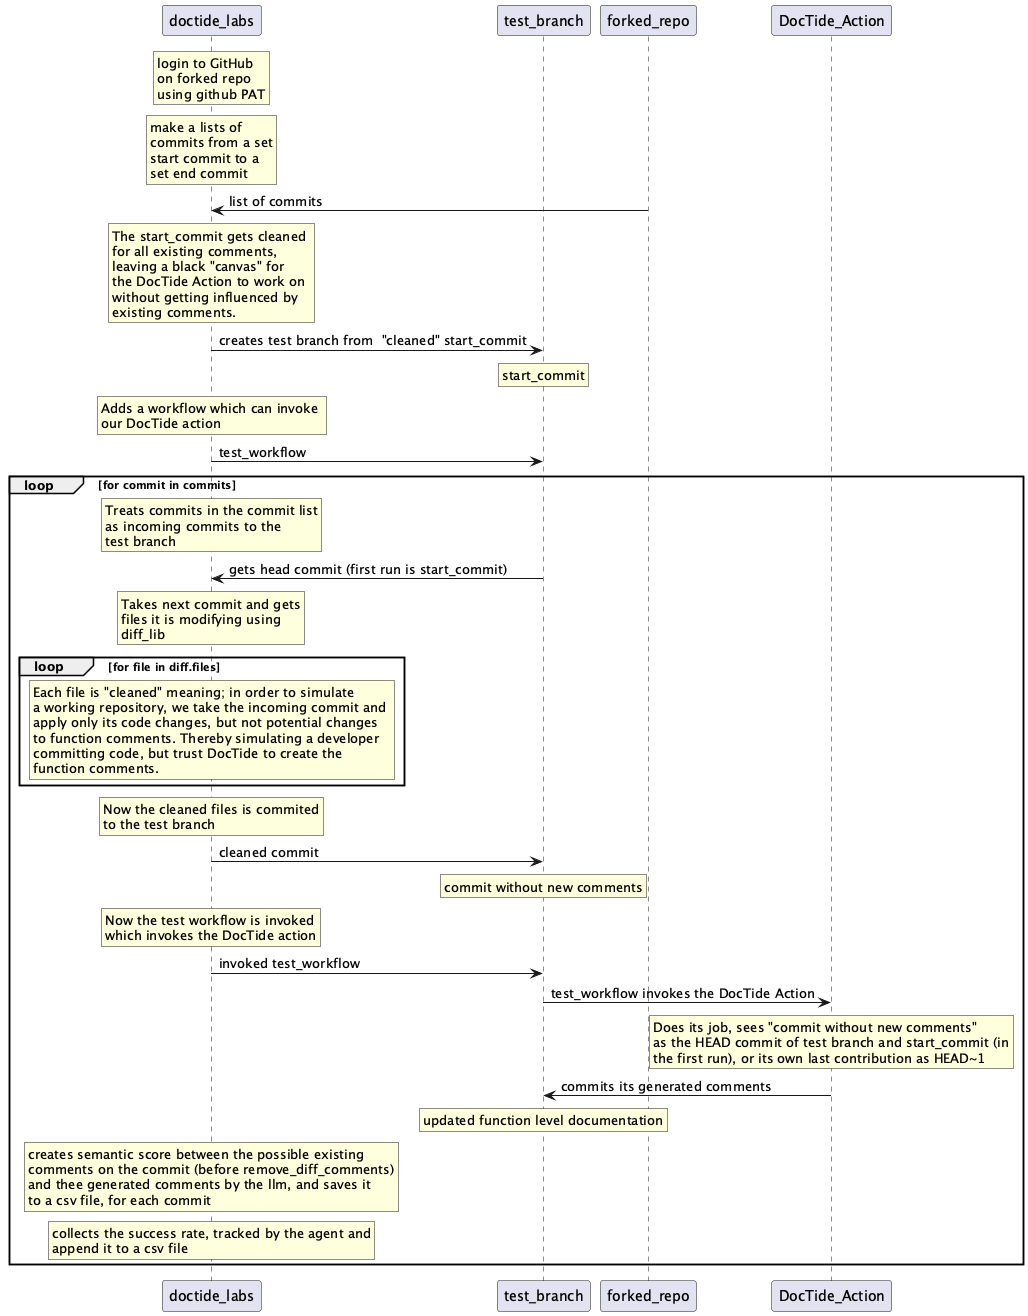
\includegraphics[width=0.7\linewidth]{Figures/doctide_labs_flow_chart.png}
\caption{The flow of the state the evaluation setup has, how commits are collected from a repository, preprocessed, and then committed to the test-branch, where DocTide is invoked, and finally metrics are collected}
\label{fig:flow_labs}
\end{figure}
    \item Technical description of DocTide Labs as Real World Simulation Protocol
    \item data collection
    \item Data pre-processing 
\end{itemize}
\textbf{Q3: }What are the challenges when developing and integrating an autonomous agent into GitHub Action?\textcolor{red}{or CI?}